Wix~\cite{wix}, similarly to Squarespace (mentioned in a prior section of this overview), mainly offers a website building service which enables users to create their own websites using the Wix Website Builder UI. When building a website, users can make use of the so-called Wix Apps found in the Wix App Market. These can be thought of as plugins/extensions that the user can use to add functionality to their website or to the administrative dashboard. Wix Apps can be either official ones developed by Wix, or third-party ones (Wix provides an extensive API and even options to monetize the Apps published in the Wix App Market).

Wix offers three official Wix Apps which can in various ways be used to add reservation functionality to a Wix website: Wix Bookings, Wix Events, and Wix Restaurants. Wix Bookings seems to be meant for businesses offering frequently occurring appointments or classes. Wix Events appears more suited for those who organize events that only happen a few times or infrequently (Wix~\cite{wix} lists \enquote{planning a wedding, hosting a convention, or selling tickets to a show} as examples). Wix Restaurants, as the name suggests, focuses purely on restaurant businesses, enabling them to for example showcase their menu, receive orders, but also to set up online reservations.

This overview focuses on Wix Events, which are available as part of Wix's free plan (with some limitations), and briefly on Wix Bookings, which do not work with the website as part of the free plan, but do at least let users set up the administrative section.

After first signing up for an account, Wix asks the user a few questions about the purpose of their website to be built. Based on these answers it customizes the UI a bit, including adding suitable Wix Apps. When choosing the \enquote{Book Event} option as the primary focus of the website, the user is directed into the setup of the already installed Wix Events. They create their first event by entering the following:
\begin{itemize}
    \item the name of the event,
    \item the type of the event -- either a \enquote{Ticketed event} with options for pricing and availability or a \enquote{Registration only} event meant to collect confirmations of an invitation (RSVPs),
    \item the starting time and date of the event,
    \item optionally the ending time and date of the event,
    \item whether it is a recurring event (this lets the user add multiple dates/times for the event, but there does not appear to be an option to do this automatically),
    \item and optionally the location of the event (which can be a physical address or online).
\end{itemize}

The user can then add various tools to their website. These tools include for example a seating map which can \enquote{let guests choose their seats} or email marketing which can send invitations.

Lastly, the user can set up a custom domain to use for their website (though this is only available with a paid plan; otherwise the service provides a free Wix subdomain), design their website, and optionally optimize the website's SEO. If the user selected the \textit{Ticketed} event type, they also need to create ticket types for the created event to be bookable.

For designing the website, there are ready-made layouts which can be customized to a great extent, since that is Wix's primary focus. The user can also let the service use artificial intelligence (AI) to generate the website layout for them. Since this overview's goal is not to evaluate website builders, the AI option was chosen to save time. The resulting layout appeared fairly usable, though it seemed to have issues adjusting to different window sizes.

In the event details, the user can additionally provide a description and an image for the event. Events can be grouped into categories. Creating a ticket asks for the name of the ticket, optionally its description, the number of tickets available, a pricing method, and a window of time when the ticket is available for purchase. Tickets can be limited to a maximum amount per single order.

The pricing method can be fixed to a certain amount, split into different categories (e.g. child, adult), \enquote{pay what you want,} and free. Wix lets users connect third-party payment processors to collect these payments (such as PayPal and Stripe, but the availability of the payment processors depends on the user's country), and it charges a service fee (which is added on top of the payment processor's fee).

Events can have forms attached, which can include fields of multiple different data types. With the seating map tool, the user can create a detailed map of the seats and areas available at the event venue. They can then assign the available tickets to specific seats or areas. This seating map from the customer's perspective can be seen in the figure~\ref{fig:wix_seating_map}.

When all of this is set up, the user can publish the event on their website. Customers who access the website then navigate the event, see its details (such as the name, the time and date, and the location) and available tickets. If the window, during which tickets are up for sale, is open, they choose the ticket to buy by selecting the seat or admission area from the map (or, if no seating map was added, just choose which type of ticket to buy and its quantity), fill out any form the business user attached to the event, and check out. The customer can then download their tickets as a PDF document and add the event to their personal calendar. They also receive an email with the details of their booking.

The tickets that a customer receives include a QR code in them, which can then be scanned on location by the event organizer using a special-purpose mobile app from Wix. It does not appear that a customer can reschedule or cancel their booking, though the business user can do this for them (as well as cancel the event completely) through an overview of their orders and guests, though according to Wix~\cite{wix}, they will need to handle any refunds themselves. The business user can also add guests manually and later on manually check in any guest.

The Wix Bookings App adds a section with a booking calendar to the administrative dashboard. The user can add a service they would like to provide to their customers, which can be either an appointment (described as \enquote{a private session that can be booked according to availability}), a class (described as \enquote{a group session that can recur} where \enquote{clients book any session they want to join}), or a course (described as \enquote{a set of group sessions} where \enquote{clients book them all up front}).

In addition to providing some basic details about the service, the user can add pricing or a long-term membership plan, as well as staff members who provide the service. A booking form can also be attached. Unlike with Wix Events, the booking can be canceled or rescheduled by the customers, since there are options to disable this and limit the period of time before the booking when such changes can be made. Additionally, there is an option to require manually accepting all bookings.

The business user also sets up their opening hours, so that the service can offer recurring classes during these times (unlike with Wix Events, where recurring events had to have their times and dates added manually). A useful feature is also the option to schedule the appointment time slots either based on the service duration or every fixed amount of time. Booking reminders through email and SMS, calendar synchronization, and waiting lists are available as well. An example of a Wix website with the Wix Bookings functionality can be seen in the figure~\ref{fig:wix_bookings}.

Other features of the platform include built-in website analytics, multiple staff members managing a single account with role-based permissions, business website localization, CSV export of orders, and a full-featured API.

\begin{figure}
    \centering
    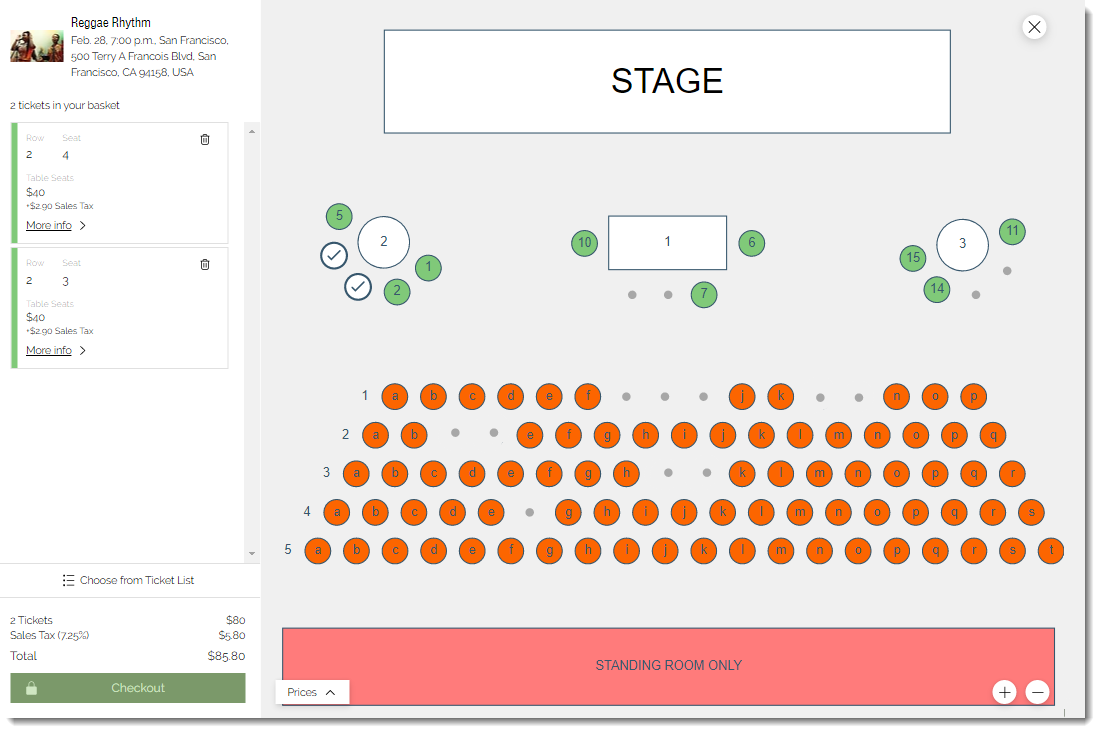
\includegraphics[width=1.0\textwidth]{content/existing_reservation_systems/wix_seating_map.png}
    \caption[Wix Events]{Wix Events~\cite{wix}}
    \label{fig:wix_seating_map}
\end{figure}

\begin{figure}
    \centering
    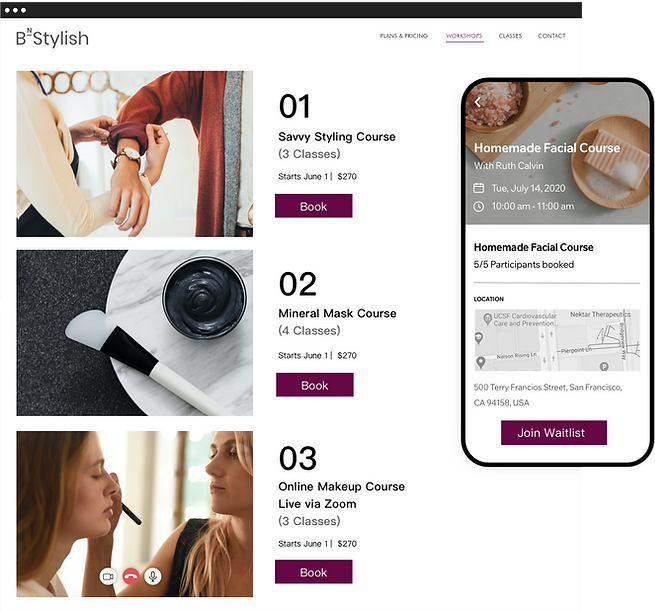
\includegraphics[width=1.0\textwidth]{content/existing_reservation_systems/wix_bookings.png}
    \caption[Wix Bookings]{Wix Bookings~\cite{wix}}
    \label{fig:wix_bookings}
\end{figure}
